
%\documentclass[14pt]{extarticle}
\documentclass[12pt,a4paper]{scrbook}
\usepackage[cm-default]{fontspec}
\usepackage{csquotes}
\usepackage{url}
\usepackage[shortcuts]{extdash}
\usepackage{pgffor}
\usepackage[unicode=true]{hyperref}
%\usepackage{breakurl}
\usepackage{array}
%\usepackage{graphicx}
\usepackage[export]{adjustbox}
\usepackage{listings}
\renewcommand{\lstlistingname}{\inputencoding{latin0}Listing}

\usepackage{xcolor}

\usepackage{polyglossia,xunicode}
\setdefaultlanguage{english}
\setotherlanguage{tamil}
\setotherlanguage{portuguese}

\usepackage[normalem]{ulem}
%\usepackage[noend,noeledsec,noledgroup]{reledmac}
\renewcommand{\multfootsep}{\,}
\usepackage[margin=1in]{geometry}

\usepackage{footnote}
\makesavenoteenv{tabular}

\usepackage{setspace}
\onehalfspacing

\graphicspath{ {./assets/} {./img/} }

\usepackage{changepage}

\setlength{\parskip}{\medskipamount}
\setlength{\parindent}{0pt}

\setmainlanguage{english}
\setotherlanguage{tamil}
\setmainfont[
    Path = ./fonts/brill-typeface/,
    UprightFont = brill-roman,
    BoldFont = brill-bold,
    ItalicFont = brill-italic,
    BoldItalicFont = brill-bold-italic,
    Extension = .ttf]{Brill}
\newfontfamily{\defaultfont}[
    Path = ./fonts/brill-typeface/,
    UprightFont = brill-roman,
    BoldFont = brill-bold,
    ItalicFont = brill-italic,
    BoldItalicFont = brill-bold-italic,
    Extension = .ttf]{Brill}
\newfontfamily{\tamilfont}[
    Path = ./fonts/,
    Script = Tamil,
    Language = Tamil,
    UprightFont = *,
    UprightFeatures = {RawFeature={+axis={wght=300}}},
    BoldFont = *,
    BoldFeatures = {RawFeature={+axis={wght=500}}},
    Extension = .otf]{TSTTamil}

\usepackage[Tamil,Latin]{ucharclasses}
\setDefaultTransitions{\defaultfont}{}
\setTransitionsForLatin{\defaultfont}{}
\setTransitionTo{Tamil}{\tamilfont}

%\usepackage[style=chicago-authordate,natbib=true,backend=biber,maxcitenames=2]{biblatex}
%\usepackage{cite}

\begin{document}
    \begin{titlepage}

    \title{\emph{Tamil grammar in Portugese}}\subtitle{A diplomatic edition of Indien 188c, Bibliothèque nationale de France}\author{Cristina MURU}
\date{}
\publishers{
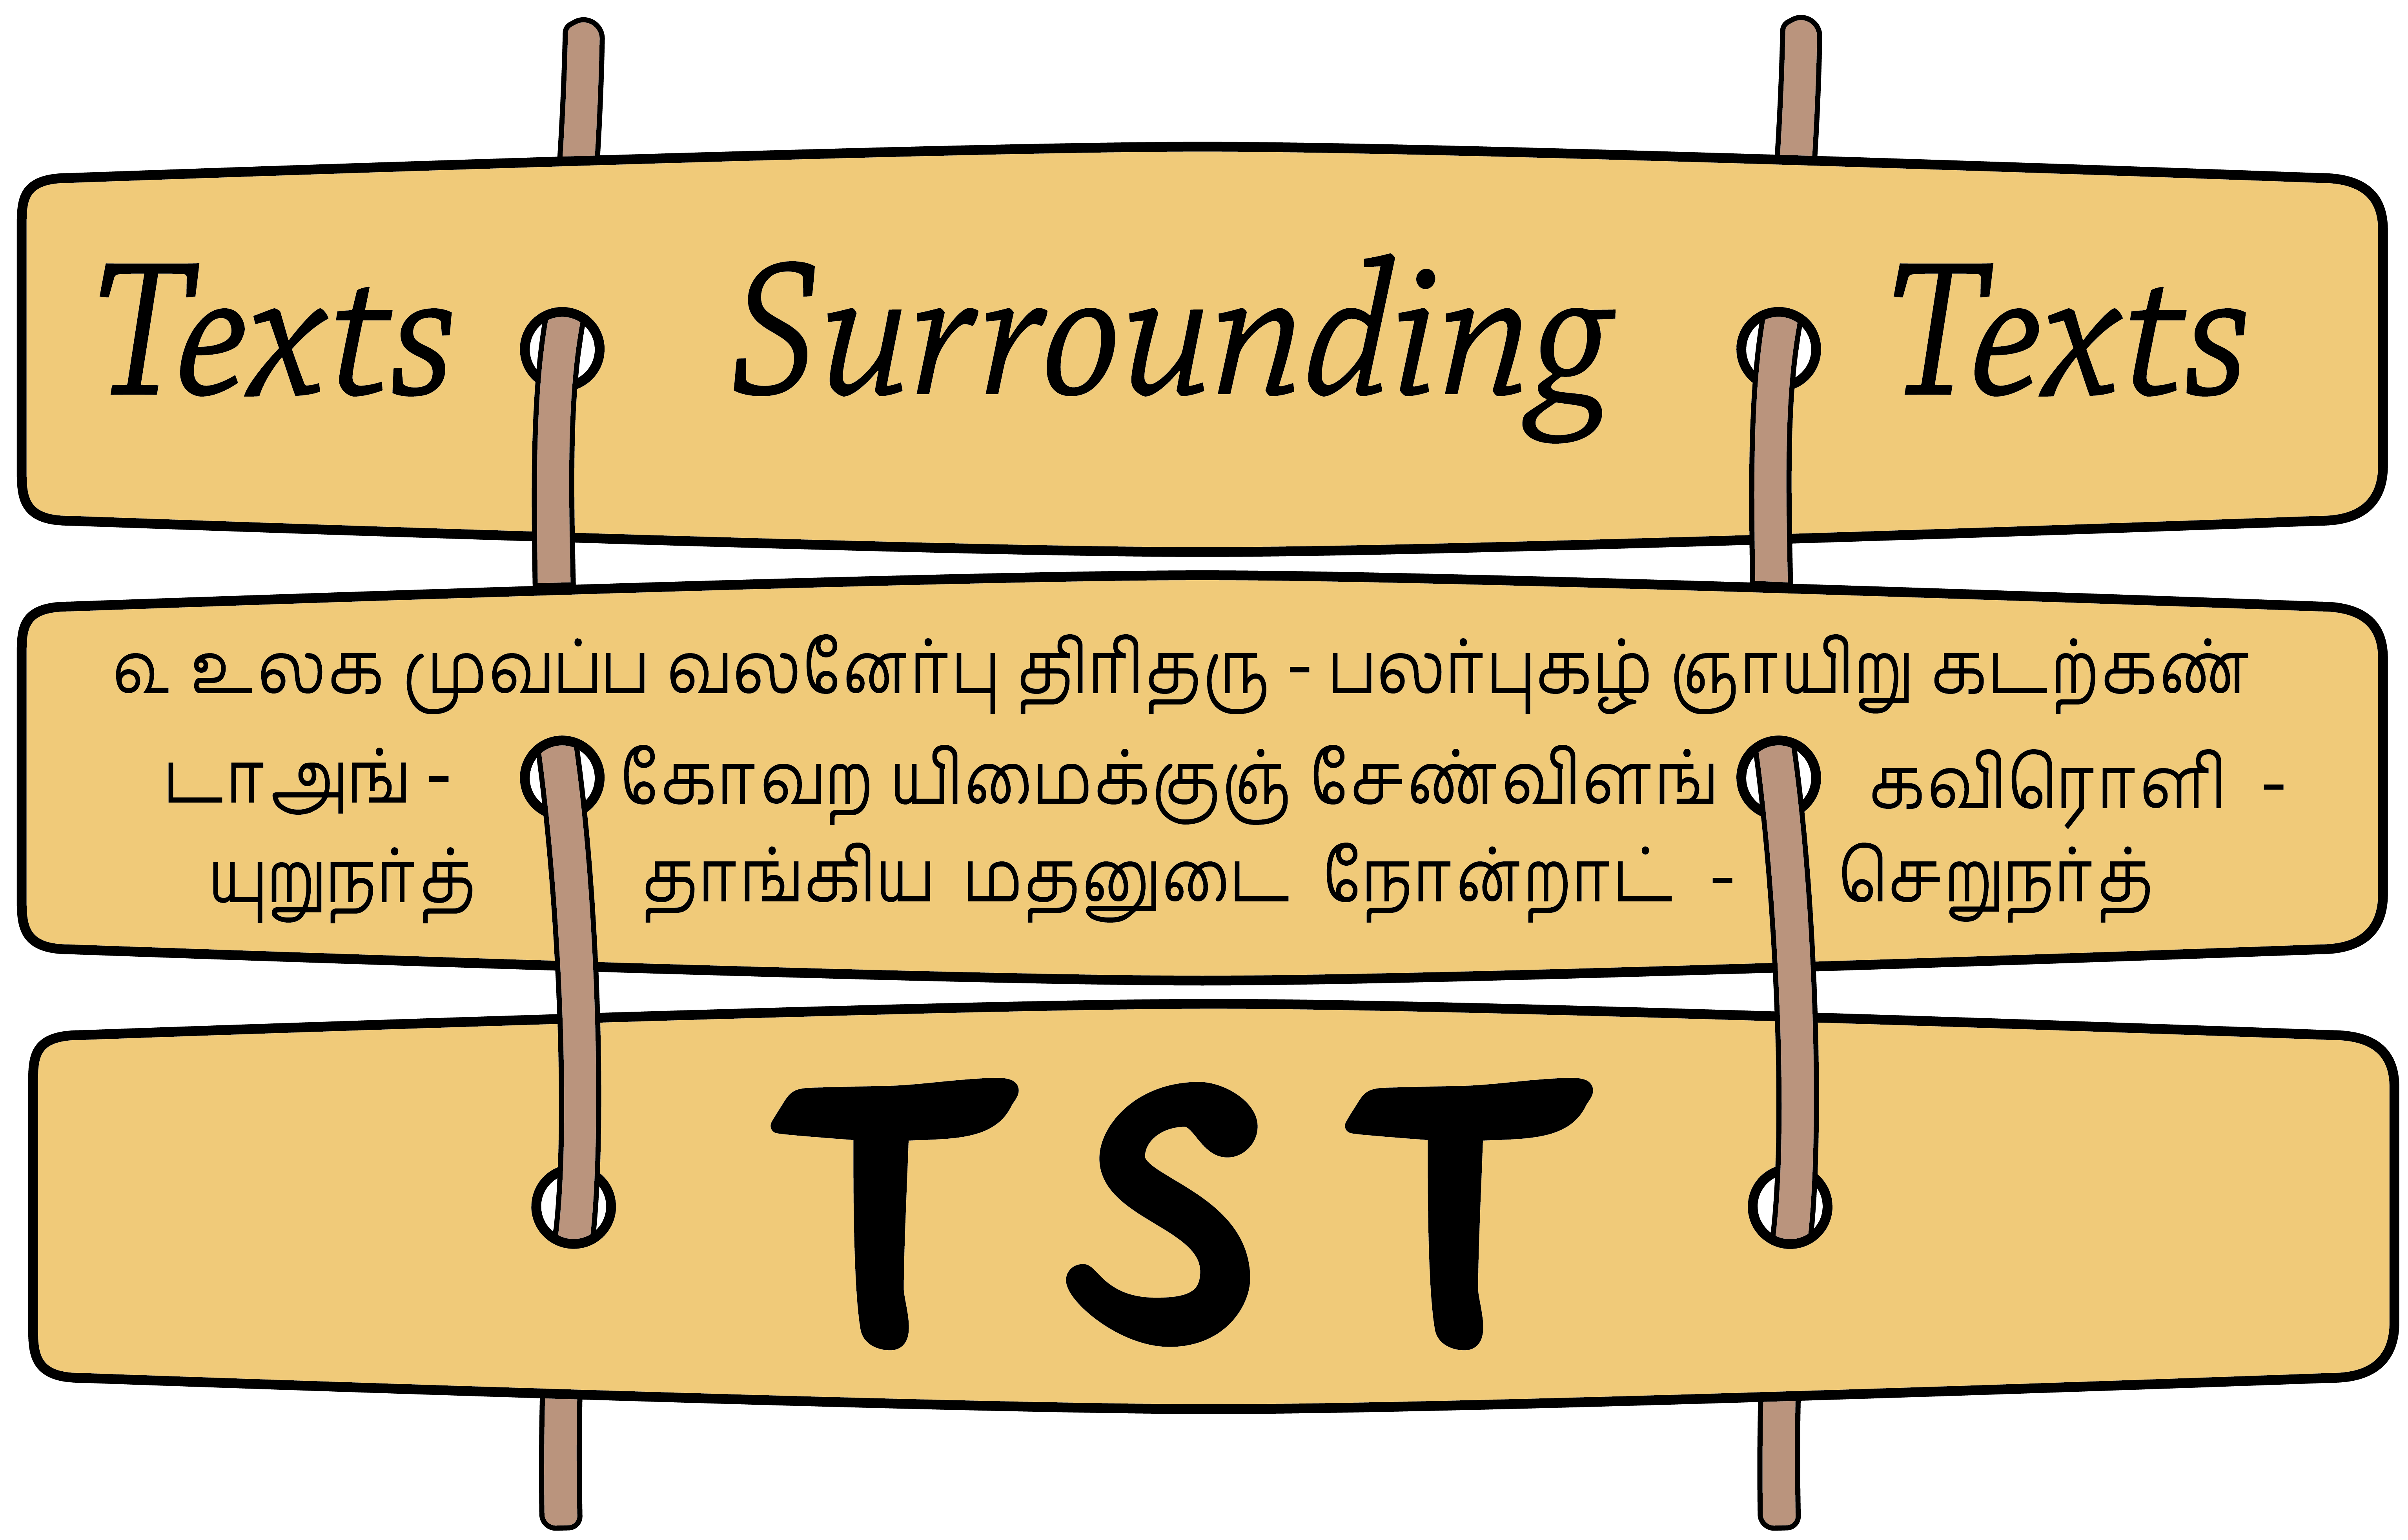
\includegraphics[height=2em]{tst}\\
Texts Surrounding Texts\\
Paris · Hamburg
}   
\end{titlepage}
    
\lowertitleback{
    
\includegraphics[height=1em]{cc.xlarge} 
\includegraphics[height=1em]{by.xlarge} 
\includegraphics[height=1em]{nc-eu.xlarge} 2022 Cristina MURU\\
    This text is licensed under a Creative Commons Attribution-NonCommercial license.\\
    Manuscript images are courtesy of Gallica / Bibliothèque nationale de France.\\
    \\
    ISBN XXXX-XXXX-XXXX eBook\\
    \\
    Text Surrounding Texts (FRAL 2018, ANR/DFG)\\
    Centre nationale de la recherche scientifique\\
    Paris, France\\
    \\
    
\includegraphics[height=2em]{anr} \hfill 
\includegraphics[height=2em]{bnf} \hfill 
\includegraphics[height=1.8em]{dfg} \\
}
    \maketitle
    \newpage
    \begin{center}\textsc{TST Diplomatic Editions}\\

    \quotation{This edition has been published as part of the Texts Surrounding Texts project, funded jointly by the Agence nationale de la recherche in France and the Deutsche Forschungsgemeinschaft in Germany. TST Diplomatic Editions publishes unique and important manuscripts from the collection of the Bibliothèque nationale de France.}
    \end{center}
    
\newpage

\tableofcontents

\part{Introduction}
    
\part{The manuscript}
\newpage
                       

A grammar of Tamil language in Portuguese, containing descriptions and explanations about declensions, conjugation and syntax.
                     
\begin{itemize}
    
                         
\item First come the declensions (\hyperlink{img-25}{f8r}‒\hyperlink{img-35}{f13r}). The nouns chosen for illustrating the declensions are the same as those found in \emph{Arte da lingua Malabar} composed around 1549 by the Jesuit Henrique Henriques (1520‒1600). For instance, the first declension of Henriques corresponds to the sixth declension here; the third to the fourth; the fourth to the first; and the fifth to the third. The second declension is the same in both.
    
                         
\item We find afterwards explanations about nouns and adjectives, e.g.: “os nomes acabados em ஆ â (…)” (\hyperlink{img-37}{f14r}); “dos Nomes adiectiuos” (\hyperlink{img-39}{f15r}); “dos Comparatiuos” (\hyperlink{img-41}{f16v}); “dos Superlatiuos” (\hyperlink{img-43}{f17r}); “dos nomens de qualidade et gantidade” (\hyperlink{img-44}{f17v}); “pera os nomens de quantidade” (\hyperlink{img-45}{f18r}\hyperlink{img-46}{v}) ; “dos nomens Numerais” (\hyperlink{img-47}{f19r}‒\hyperlink{img-50}{20v}) ; “dos pronomens” (\hyperlink{img-51}{f21r5}).
    
                         
\item Then comes the book II on verbs (“Livro 2° dos uerbos,” (\hyperlink{img-57}{f24r}). The following headears are found in this portion of the text: “primeira Conjugacaó” (\hyperlink{img-57}{f24r}); “2a Conjugacaó” (\hyperlink{img-69}{f30r}); “3a Conjugacaó” (\hyperlink{img-79}{f35r}); “4a Conjugacaó” (\hyperlink{img-83}{f37r}); “5a Conjugacaó” (\hyperlink{img-87}{f39r}); “dos uerbos Compositos” (\hyperlink{img-91}{f41r}); “dos uerbos passiuos” (\hyperlink{img-91}{f41v11}); “Dos uerbos Impersoaes” (\hyperlink{img-93}{f42r1}); “dos uerbos defeitivo”” (\hyperlink{img-96}{f43v17}).
    
                     
\item Finally from \hyperlink{img-100}{f45v}, various topics are discussed, e.g.: “dos participios” (\hyperlink{img-100}{f45v}); “do casu” (\hyperlink{img-100}{f45v}); “do Dativo” (\hyperlink{img-102}{f46v}); “por Accusativo” (\hyperlink{img-103}{f47r}); “por ablatiuo” (\hyperlink{img-104}{f47v}); “dos participios directiuos” (\hyperlink{img-108}{f49v}); “dos participios do Infinito” (\hyperlink{img-108}{f49v}); “dos tempos menos principaes” (\hyperlink{img-109}{f50r}); “da particula, Am” (\hyperlink{img-114}{f52v}); “das proposicoens” (\hyperlink{img-116}{f53v}); “aduerbios de tempo” (\hyperlink{img-118}{f54v}); “de responder” (\hyperlink{img-119}{f55r}); “de afirmar” (\hyperlink{img-119}{f55r}); “de negar” (\hyperlink{img-119}{f55r}); “de quandidade” (\hyperlink{img-121}{f56r}); “modo de formar os uerbos” (\hyperlink{img-122}{f56v}).
    
                         
\item The last folio is about “de quantitade” (\hyperlink{img-121}{f56r}). The \hyperlink{img-123}{f57v} bears a crossed-out word.
    
                        
\end{itemize}
    
                    
\cleardoublepage
\makeatletter\@openrightfalse
\part{Diplomatic edition}
    
    
    	
\newpage
\hypertarget{img-25}{
    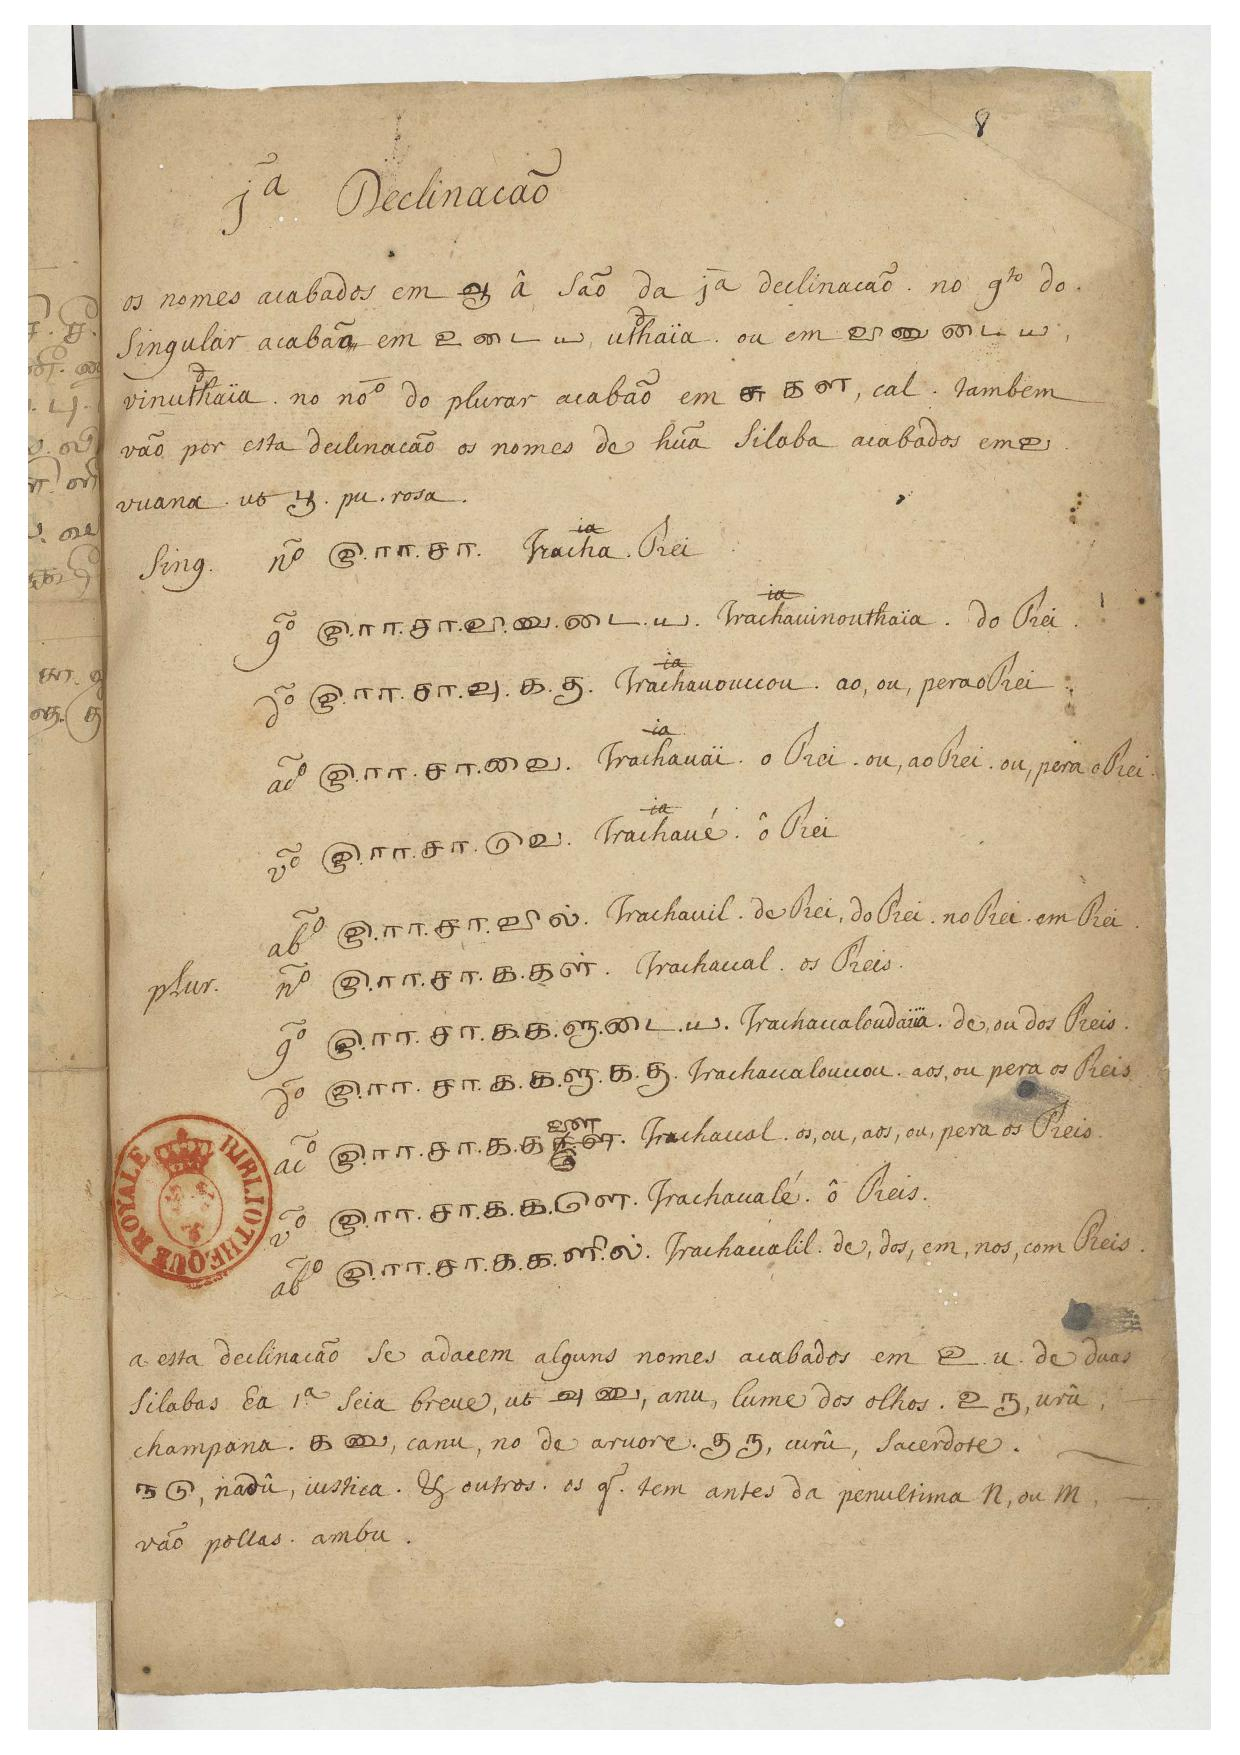
\includegraphics[width=\textwidth]{img-25}}
\newpage
        \chapter*{1° Declinacaõ}
    \addcontentsline{toc}{chapter}{1° Declinacaõ}
    
        


            Os nomes acabados em ஆ â saõ da 1° declinaçaõ no g[enitiv]o do 
            singular acabã em உடைய uthaïa ou em வினுடய
            vinuthaïa no n[ominativ]o do plural acabaõ em ககள cal . Tambem
            vaõ por esta declinacaõ os nomes e huã silaba acabados em வ
            vuana ut பூ pu.rosa. 
        
        
\begin{tabular}{lllll}
    
            
                Sing. &
                n\textsuperscript{õ} &
                இ.ரா.சா. &
                iracha &
                Rei \\
    
            
    
            
                 &
                g\textsuperscript{õ} &
                இ.ரா.சா.வினு.டை.ய &
                irachavinouthaïa &
                do Rei \\
    
            
    
            
                 &
                d\textsuperscript{õ} &
                இ.ரா.சா.வு.ககு &
                irachavouccou &
                au, ou, pera o Rei \\
    
            
    
            
                 &
                ac\textsuperscript{õ} &
                இ.ரா.சா.வை &
                irachavaï &
                o Rei, ou, ao Rei, ou, pera o Rei \\
    
            
    
            
                 &
                v\textsuperscript{õ} &
                இ.ரா.சா.வெ &
                irachavé &
                ô Rei \\
    
            
    
            
                 &
                ab\textsuperscript{õ} &
                இ.ரா.சா.வில &
                irachavil  &
                de Rei, do Rei, no Rei, em Rei \\
    
            
    
            
                plur. &
                n\textsuperscript{õ} &
                இ.ரா.சா.ககள &
                irachaccal &
                os Reis \\
    
            
    
            
                 &
                g\textsuperscript{õ} &
                இ.ரா.சா.க்களு.டை.ய &
                irachaccaloudaïa  &
                de ou dos Reis \\
    
            
    
            
                 &
                d\textsuperscript{õ} &
                இ.ரா.சா.க.க.ளு.க.கு &
                irachaccalouccou &
                aos, ou pera os Reis \\
    
            
    
            
                 &
                ac\textsuperscript{õ}\footnote{In prima istanza scrive iracchacaḷ, poi corretto in -cale, infine con -caḷai. In uso vecchia legatura per la rappresentazione di ḷ+ai.} &
                இ.ரா.சா.க.க.ளை &
                irachaccal &
                os, ou, aos, ou, pera os Reis \\
    
            
    
            
                 &
                v\textsuperscript{õ} &
                இ.ரா.சா.க.க.ளெ &
                irachaccalé &
                ô Reis \\
    
            
    
            
                 &
                ab\textsuperscript{õ} &
                இ.ரா.சா.க.க.ளல &
                irachaccalil  &
                de, dos, em, nos, com Reis \\
    
            
    
        
\end{tabular}
    
        

a esta declinacaõ se adacem alguns nomes acabados em உ u de doas silabas e a 1° seia breve, ut அனு, anu, lume dos olhos, உரு, urû, champana, கனு, canu, no de arvore. குரு, curû, sacerdote. நடு, nadû, iustica. Et outros os q[uaes] tem antes da penultima n, ou m, vaõ pollas amba.
        
        
\newpage
\hypertarget{img-27}{
    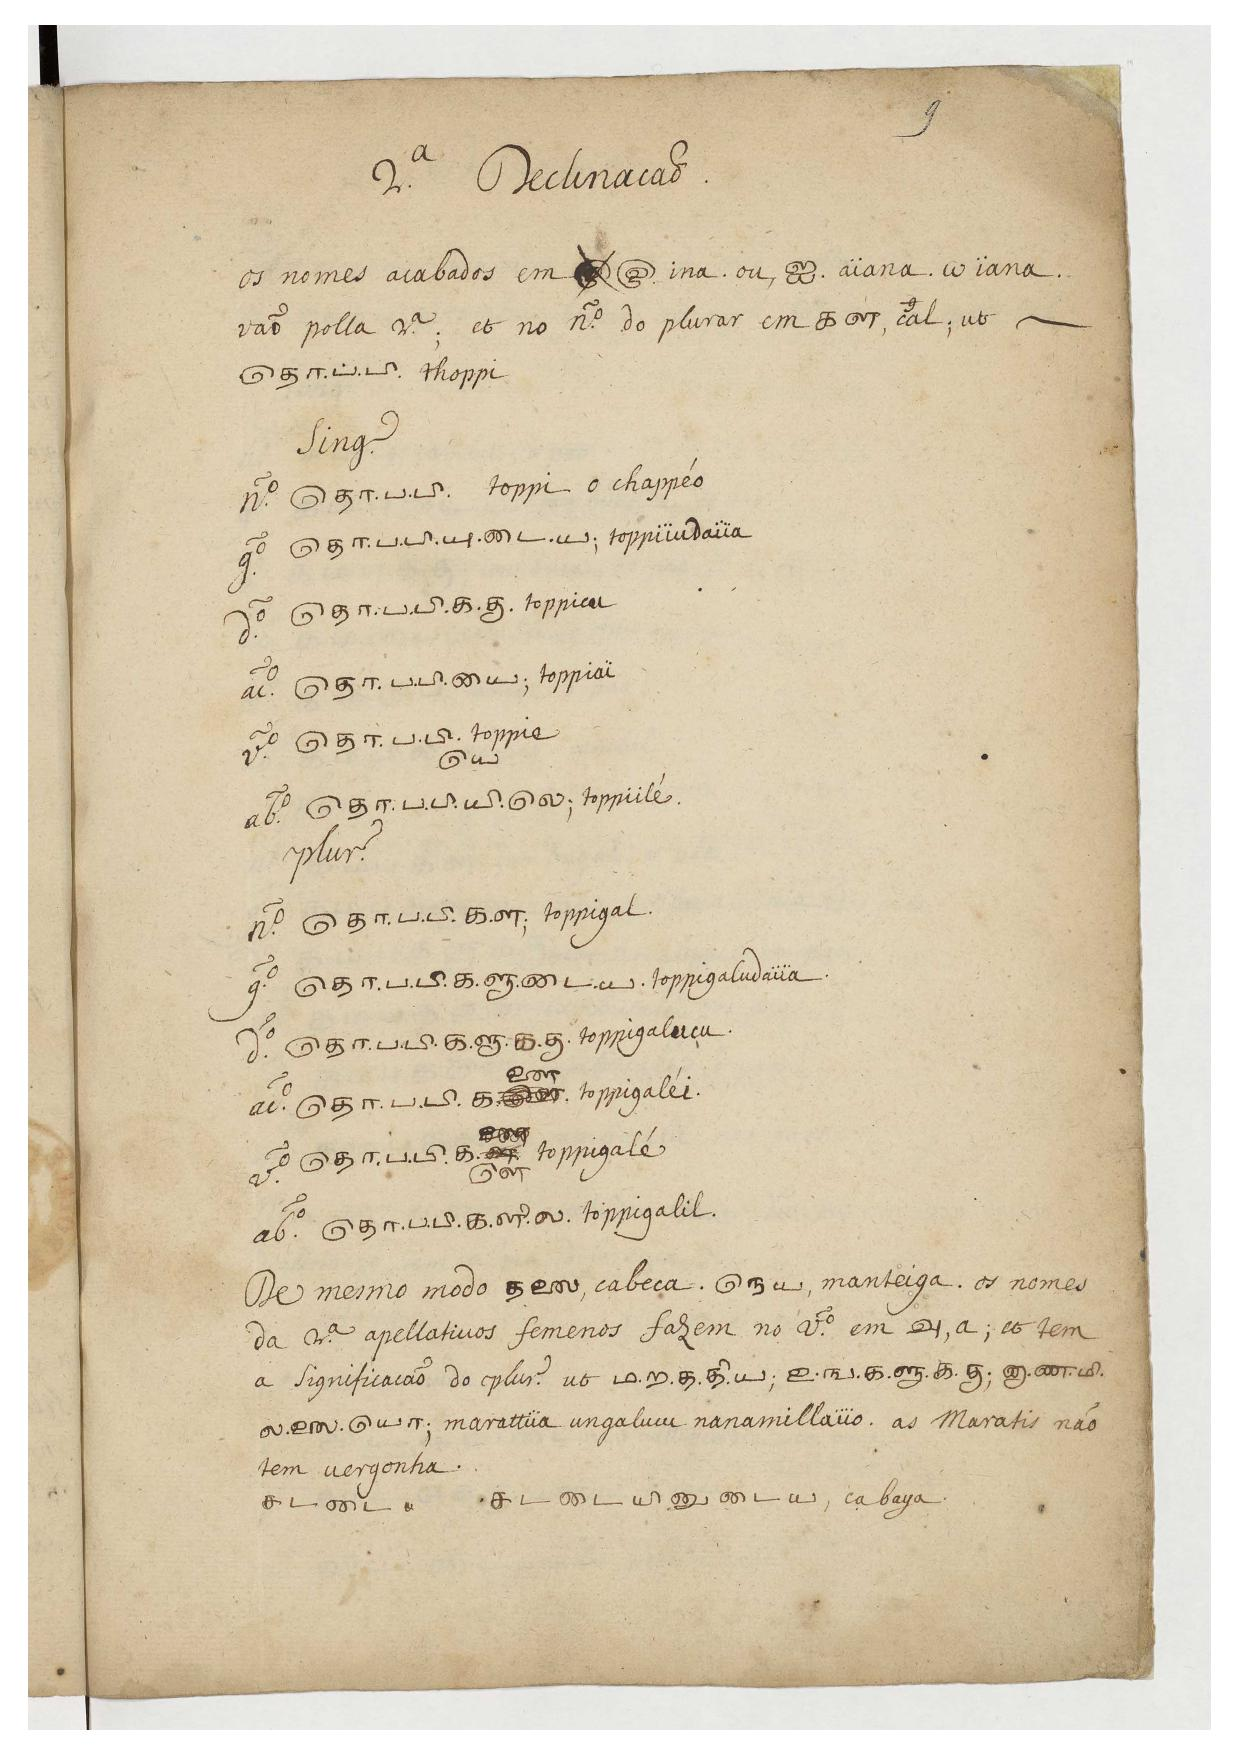
\includegraphics[width=\textwidth]{img-27}}
\newpage
        \chapter*{2° Declinacaõ}
    \addcontentsline{toc}{chapter}{2° Declinacaõ}
    
        


            os nomes acabados am \sout{\textcolor{gray}{இ}}இ ina, ou ஐ, aïana, ய, ïana 
            vaõ polla 2° et no n[ominativ]o do plurar em கள cal, 
            ut தொ.ப்.பி thoppi.
        
        
\begin{tabular}{lllll}
    
            
                Sing. &
                n\textsuperscript{õ} &
                தொ.ப.பி &
                toppi &
                o chappéo \\
    
            
    
            
                 &
                g\textsuperscript{õ} &
                தொ.ப.பி.யு.டை.ய &
                toppïïudaïa &
                 \\
    
            
    
            
                 &
                d\textsuperscript{õ} &
                தொ.ப.பி.க.கு &
                toppicu &
                 \\
    
            
    
            
                 &
                ac\textsuperscript{õ} &
                தொ.ப.பி.யை &
                toppiaï &
                 \\
    
            
    
            
                 &
                v\textsuperscript{õ} &
                தொ.ப.பி.யெ &
                toppia &
                 \\
    
            
    
            
                 &
                ab\textsuperscript{õ} &
                தொ.ப.பி.யி.லெ &
                toppilé &
                 \\
    
            
    
            
                plur. &
                n\textsuperscript{õ} &
                தொ.ப.பி.க.ள &
                toppigal &
                 \\
    
            
    
            
                 &
                g\textsuperscript{õ} &
                தொ.ப.பி.க.ளு.டை.ய &
                toppigaludaïa &
                 \\
    
            
    
            
                 &
                d\textsuperscript{õ} &
                தொ.ப.பி.க.ளு.க.கு &
                toppigalucu &
                 \\
    
            
    
            
                 &
                ac\textsuperscript{õ} &
                தொ.ப.பி.க.\sout{\textcolor{gray}{ளெ}}\textbf{ளை} &
                toppigaléi &
                 \\
    
            
    
            
                 &
                v\textsuperscript{õ} &
                தொ.ப.பி.க.\sout{\textcolor{gray}{ள}}\sout{\textcolor{gray}{\textbf{ளை}}}\textbf{ளெ} &
                toppigalé &
                 \\
    
            
    
            
                 &
                ab\textsuperscript{õ} &
                தொ.ப.பி.க.ளி.ல &
                toppigalil &
                 \\
    
            
    
        
\end{tabular}
    
        


            de mesmo modo தலை cabeca. நெய manteiga. Os nomes 
            \textcolor{purple}{¿}da\textcolor{purple}{?} 2° appellativos femenos fazem no v[ocativ]o em அ, a; et tem
            a significacaõ do plural ut ம.ற.த.தி.ய, உ.ங.க.ளு.க.கு, னா.ண.மி.
            ல.லை.யொ; marattïa ungaluccu nanamillaïïo, as Maratis naõ tem vergonha.
        
        


            சடடை சடடையினுடைய cabaya
        
    
   
\@openrighttrue\makeatother
    
\end{document}
    
